\documentclass[11pt]{article}
\usepackage[margin=1in]{geometry}
\usepackage{amsmath,amssymb}
\usepackage{booktabs}
\usepackage{graphicx}
\usepackage{tabularx}
\usepackage{array}
\usepackage{hyperref}
\usepackage[T1]{fontenc}
\usepackage{caption}
\usepackage{xurl}

\newcolumntype{Y}{>{\raggedright\arraybackslash}X}
\newcolumntype{P}[1]{>{\raggedright\arraybackslash}p{#1}}

\hypersetup{colorlinks=true,linkcolor=blue,urlcolor=blue}
\graphicspath{{./}}
\setlength{\parindent}{0pt}
\setlength{\parskip}{0.55em}
\captionsetup{font=small,skip=6pt}

\title{What is in this \texttt{results} folder}
\author{MUERP / SeQUeNCe experiments}
\date{November 10, 2026}

\begin{document}
\maketitle

This folder holds the \textbf{output} of three experiments.
You do not need to run any code to read it.
The inputs live one directory up (\texttt{muerp/algorithms.py}, \texttt{run\_sweeps.py}, \texttt{mc\_physics.py}, \texttt{inject\_alg4\_coherence.py}).

Compile this file from \emph{this} directory:
\begin{verbatim}
pdflatex README.tex
\end{verbatim}

\section{The one-sentence context}

A 2024 paper (Zeng et al., ICDCS) studies \textbf{MUERP}: how several users in a quantum network should share limited switch memory in order to become entangled with each other.
The paper's plotted number is a one-shot success probability $P$ for a chosen set of paths (an \emph{entanglement tree}).
We asked whether the open-source simulator \textbf{SeQUeNCe} can host that problem.
The files here are the numbers and plots from that check.

\section{Two different kinds of number}

Do not mix them.

{\small
\begin{tabularx}{\textwidth}{@{}P{1.35in} Y@{}}
\toprule
Kind & Meaning \\
\midrule
\textbf{Slot $P$}
  & Probability that every link and every swap in the tree succeeds \emph{once}, in the same time slot.
    This is what the paper plots.
    Each path of $\ell$ hops has rate $P_A = q^{\ell-1}\prod p$, then $P=\prod P_A$.
    If the tree cannot be reserved, $P=0$.
    Files: \path{figs_5_8.json}, the seven PDFs, and the analytic half of \path{mc_physics.json}. \\
\addlinespace
\textbf{SeQUeNCe throughput}
  & How many entangled pairs a \emph{timed} simulator delivered over a $0.2$\,s window, with retries.
    Not $P$. A larger counter does not mean a better tree in the paper's sense.
    Files: \path{mc_physics.json} (\texttt{sequence\_physics}) and \path{inject_alg4_coherence.json}. \\
\bottomrule
\end{tabularx}}

Default numbers used everywhere unless a plot's axis says otherwise:
$p = 0.9$ (link success), $q = 0.9$ (swap success), 10 users, 50 switches, 4 qubits per switch.

The five named curves / columns are:

\begin{itemize}
\item \textbf{Alg.~2, 3, 4} --- three heuristics from the paper for building a multi-user tree.
\item \textbf{E-Q-CAST} --- pairwise baseline (connect users along a path of consecutive pairs).
\item \textbf{N-FUSION} --- star baseline (everyone connects through one hub user).
\end{itemize}

Alg.~2--4 are the methods the paper proposes. The last two are what they compare against.

\section{File catalog}

\begin{center}
\begin{tabular}{@{}ll@{}}
\toprule
File & Produced by \\
\midrule
\texttt{figs\_5\_8.json} & \texttt{python -m muerp.run\_sweeps} \\
\texttt{fig5\_*.pdf} \ldots \texttt{fig8\_*.pdf} & \texttt{python -m muerp.plot\_figs} (reads the JSON) \\
\texttt{mc\_physics.json} & \texttt{python -m muerp.mc\_physics} \\
\texttt{inject\_alg4\_coherence.json} & \texttt{python -m muerp.inject\_alg4\_coherence} \\
\texttt{inject\_alg4\_coherence.md} & same run, human-readable summary \\
\bottomrule
\end{tabular}
\end{center}

JSON is the raw dump (means, standard deviations, counters).
PDFs are plots of the sweep JSON.
The \texttt{.md} is a short write-up of the injection experiment, not a second data source.

\section{The sweep: Figs.~5--8}

\texttt{figs\_5\_8.json} repeats the paper's Sec.~V plots as a \textbf{graph experiment}.
No photons are simulated.
A Python planner builds a tree on a random topology, then $P$ is computed from fiber lengths and $q$.
Each setting is averaged over \textbf{10} random graphs (the paper used 20).
Wall-clock was about 63 seconds.

JSON keys match the PDFs:

\begin{center}
\begin{tabular}{@{}lll@{}}
\toprule
JSON key & PDF & Horizontal axis \\
\midrule
\texttt{fig5\_topology} & \texttt{fig5\_topology.pdf} & Graph family (Waxman, Watts--Strogatz, Volchenkov*) \\
\texttt{fig6a\_users} & \texttt{fig6a\_users.pdf} & Number of users $|U|$ \\
\texttt{fig6b\_switches} & \texttt{fig6b\_switches.pdf} & Number of switches $|R|$ \\
\texttt{fig7a\_degree} & \texttt{fig7a\_degree.pdf} & Average node degree $D$ \\
\texttt{fig7b\_removed\_edges} & \texttt{fig7b\_removed.pdf} & Optical fibers deleted from a 600-edge graph \\
\texttt{fig8a\_qubits} & \texttt{fig8a\_qubits.pdf} & Qubits per switch $Q_r$ \\
\texttt{fig8b\_qswap} & \texttt{fig8b\_qswap.pdf} & Swap success $q$ \\
\bottomrule
\end{tabular}
\end{center}

Each JSON entry has \texttt{mean}, \texttt{std}, and \texttt{p\_zero} (fraction of replicas with $P=0$).

\textbf{Caveats written into the JSON \texttt{note} field.}
``Volchenkov'' here is a Barab\'asi--Albert stand-in, not the paper's original generator.
These plots measure the planner, not SeQUeNCe's entanglement-generation kernel.

\subsection{What you should see in the PDFs}

Higher is better ($P$ closer to 1).
On the default Waxman graph, Alg.~2, 3, and 4 sit on top of each other near $P\approx 0.026$, well above E-Q-CAST ($\approx 0.00062$) and N-FUSION ($\approx 0.0053$).
$P$ falls as you add users or switches, and rises as you add edges or raise $q$.
At $Q_r=2$, Alg.~4 still finds trees in our draws; the paper had said only Alg.~3 would.

\begin{figure}[h]
\centering
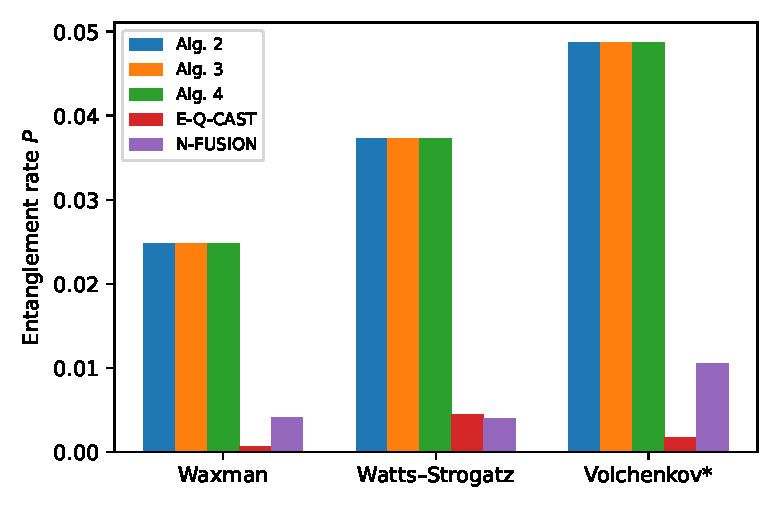
\includegraphics[width=0.72\textwidth]{fig5_topology.pdf}
\caption{\texttt{fig5\_topology.pdf}. Mean $P$ by topology. Three solid-looking bars on the left of each group are Algs.~2--4; the two remaining bars are the baselines.}
\end{figure}

\begin{figure}[h]
\centering
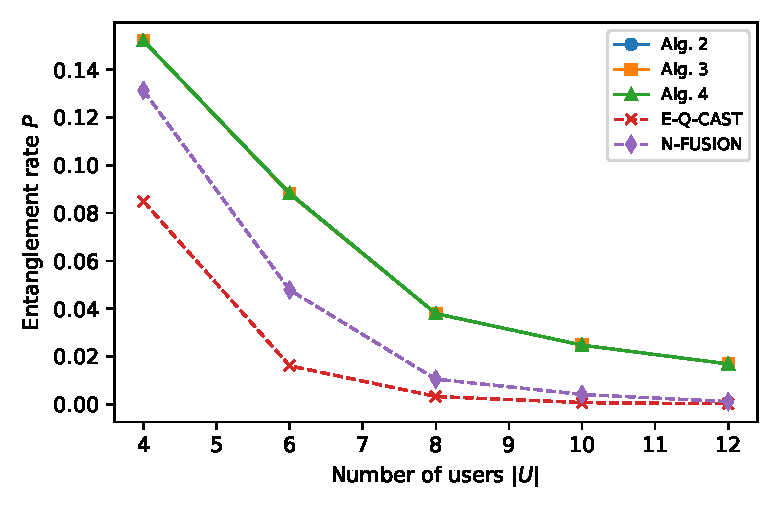
\includegraphics[width=0.48\textwidth]{fig6a_users.pdf}
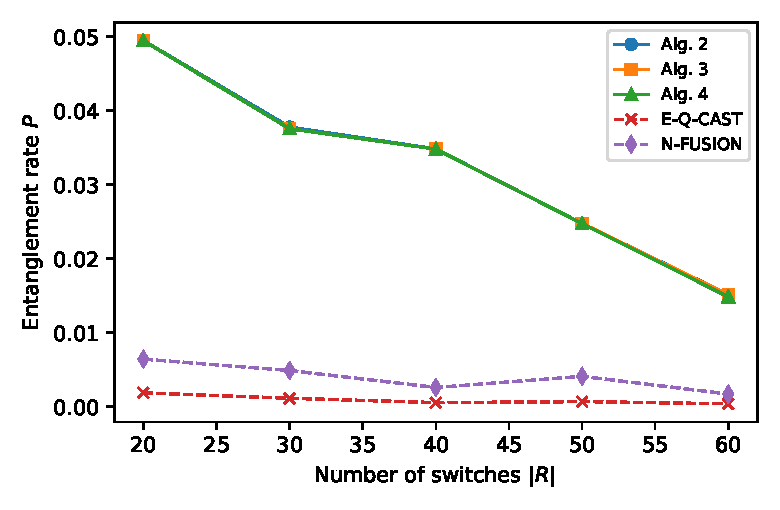
\includegraphics[width=0.48\textwidth]{fig6b_switches.pdf}
\caption{Left: \texttt{fig6a\_users.pdf} --- more users, more factors in the product $P$, so the rate drops.
Right: \texttt{fig6b\_switches.pdf} --- more switches in a fixed area lengthens typical paths.}
\end{figure}

\begin{figure}[h]
\centering
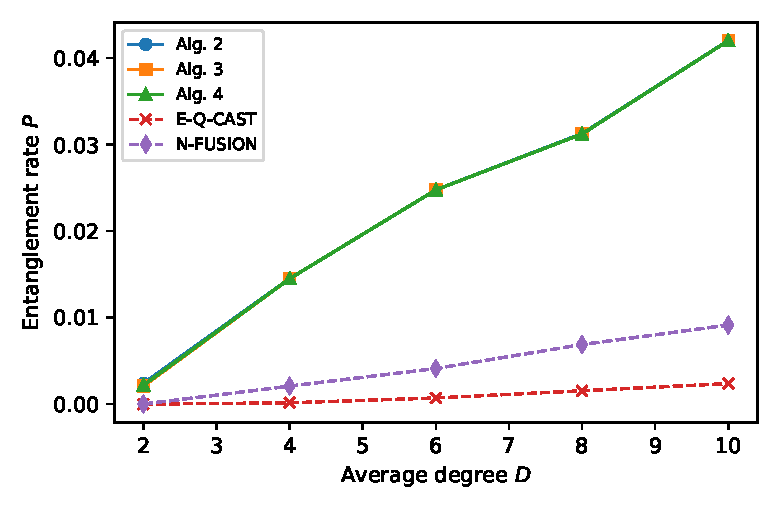
\includegraphics[width=0.48\textwidth]{fig7a_degree.pdf}
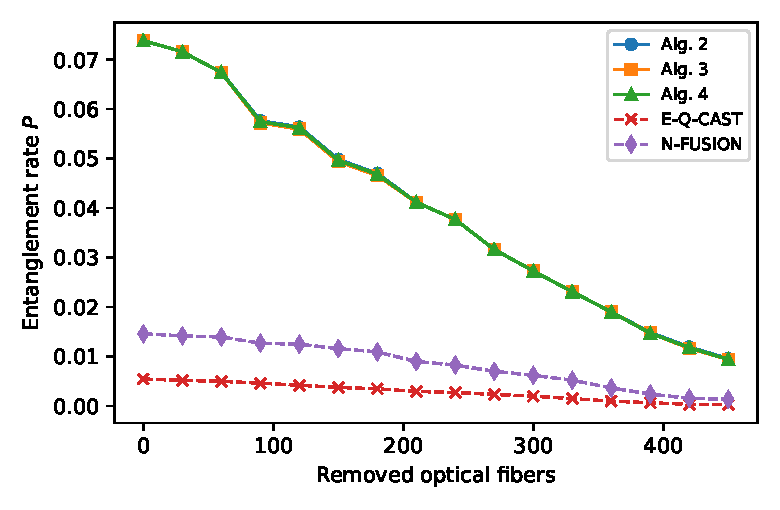
\includegraphics[width=0.48\textwidth]{fig7b_removed.pdf}
\caption{Left: \texttt{fig7a\_degree.pdf} --- sparse graphs ($D=2$) make the baselines fail.
Right: \texttt{fig7b\_removed.pdf} --- deleting fibers from a dense graph lowers $P$.}
\end{figure}

\begin{figure}[h]
\centering
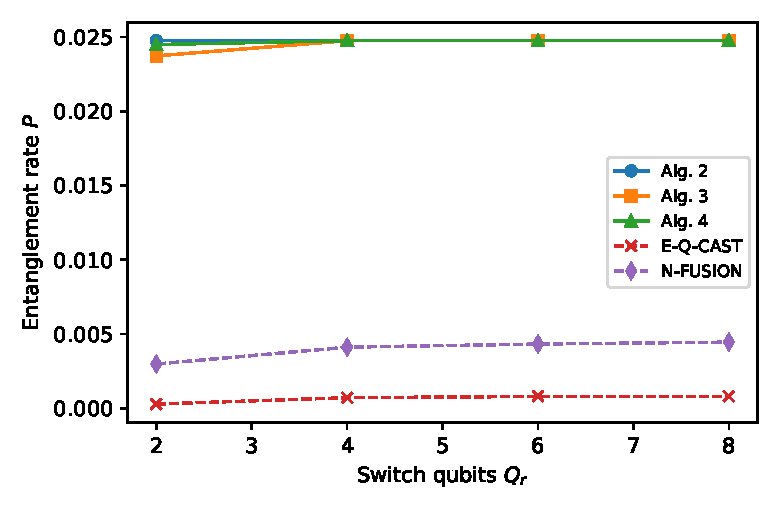
\includegraphics[width=0.48\textwidth]{fig8a_qubits.pdf}
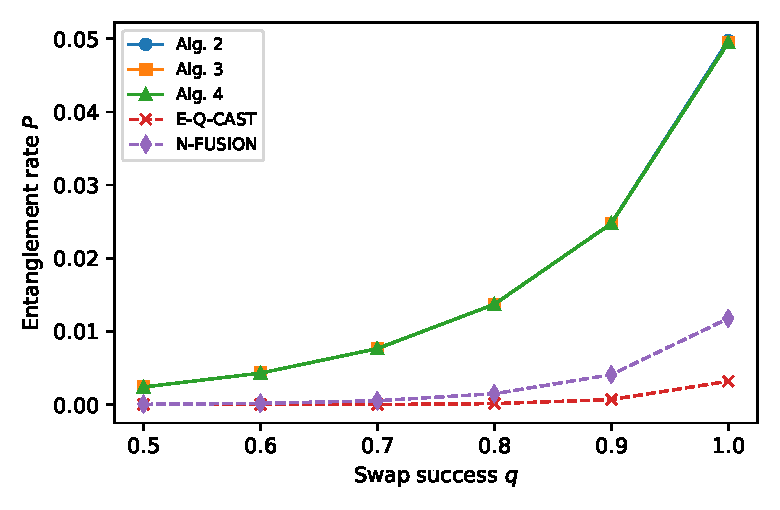
\includegraphics[width=0.48\textwidth]{fig8b_qswap.pdf}
\caption{Left: \texttt{fig8a\_qubits.pdf} --- Alg.~2 ignores the qubit budget by design, so it is flat; Algs.~3--4 meet it once $Q_r\ge 4$.
Right: \texttt{fig8b\_qswap.pdf} --- every method improves when swaps succeed more often.}
\end{figure}

\section{The small star: Monte Carlo and SeQUeNCe physics}

\texttt{mc\_physics.json} uses the paper's glossary example: three users (Alice, Bob, Carol) and one switch.
Two paths, each two links and one swap.
Analytic answer: $P = (0.9^2 \cdot 0.9)^2 = 0.531441$.

\begin{center}
\begin{tabular}{@{}ll@{}}
\toprule
Field & Value \\
\midrule
\texttt{slot\_mc.analytic\_P} & $0.531441$ (the formula) \\
\texttt{slot\_mc.mc\_mean} & $0.534$ over 20{,}000 coin-flip trials \\
\texttt{slot\_mc.mc\_std} & $0.0035$ (standard error) \\
\texttt{sequence\_physics.alice\_bob\_counter} & 7 pairs in 0.2\,s \\
\texttt{sequence\_physics.carol\_alice\_counter} & 10 pairs in 0.2\,s \\
\texttt{sequence\_physics.wall\_s} & $\approx 0.07$ seconds of real time \\
\bottomrule
\end{tabular}
\end{center}

The Monte Carlo is a sanity check that the formula is implemented correctly.
The two counters are SeQUeNCe retrying entanglement over a time window.
They are \emph{not} expected to equal $0.53$.

\section{The small star, again: pin a tree, then turn memory decay on}

\texttt{inject\_alg4\_coherence.json} asks two follow-up questions on that same three-user star.

\begin{enumerate}
\item Can we take Alg.~4's chosen paths and force SeQUeNCe's reservation protocol (RSVP) to use them?
\item If memories decohere quickly, does the \emph{reserved} tree still deliver pairs?
\end{enumerate}

\texttt{inject\_alg4\_coherence.md} is the same experiment in prose.

{\small
\begin{tabularx}{\textwidth}{@{}P{1.35in} P{1.7in} Y@{}}
\toprule
JSON object & Headline & Read as \\
\midrule
\path{admit_qs4} & Both paths reserved; RSVP matched the pin & With 4 qubits on the switch, the tree fits. Slot $P=0.531$. \\
\path{admit_qs2} & Alg.~4 returns no tree & With 2 qubits, two paths would need 4 exclusive qubits, so $P=0$. \\
\path{physics_coh_off} & Alice 7, Carol 10 delivered pairs & Infinite memory lifetime; same throughput as \path{mc_physics.json}. \\
\path{physics_coh_on} & 44 memories expired, 0 pairs delivered & $0.01$\,s lifetime. Admission is unchanged; throughput dies. \\
\bottomrule
\end{tabularx}}

Useful fields inside those objects: \texttt{rsvp\_paths\_match\_alg4} (did the simulator follow the planner), \texttt{app\_counters} (delivered pairs on each user), \texttt{memory\_expired}, \texttt{eg\_success}, \texttt{es\_success}.
Bob's counter is 0 because Bob is the \emph{responder}; SeQUeNCe counts on the initiator.

\section{What this folder is not}

\begin{itemize}
\item Not a copy of the ICDCS paper's official plots. Same axes, our graphs, 10 seeds not 20.
\item Not NetSquid. That simulator was never installed.
\item Not a 60-node photon simulation. The large-graph numbers are analytic $P$ after a planner run.
\item Not SeQUeNCe log files. Nothing here is written by SeQUeNCe itself; our scripts wrote JSON/PDF after calling it (or after not calling it, for the sweep).
\end{itemize}

For the scored write-up that uses these files, see \texttt{../muerp\_sequence\_findings.tex} (one directory above \texttt{muerp/}, in \texttt{MUERP/Simulators/}).

\end{document}
